\documentclass[12pt]{article}
\usepackage[utf8]{inputenc}
\usepackage{latexsym,amsfonts,amssymb,amsthm,amsmath}
\usepackage{float}
\usepackage{caption}
\usepackage{marginnote}
\usepackage{tikz}

\setlength{\parindent}{0in}
\setlength{\oddsidemargin}{0in}
\setlength{\textwidth}{6.5in}
\setlength{\textheight}{8.8in}
\setlength{\topmargin}{0in}
\setlength{\headheight}{18pt}

\newtheorem*{answer*}{Answer}
\newtheorem*{solution*}{Solution}
\newtheorem{remark}{Remark}

\title{Weekly Homework 5}
\author{Math Gecs}
\date{February 18, 2024}

\begin{document}
\maketitle

\subsection*{Exercise 1}
Let $f(x)$ be a a quotient of two quadratic polynomials. Given that $f(n)=n^3$ for all $n \in {1,2,3,4,5}$, compute $f(0)$.
\\

Source: Harvard-MIT Mathematics Tournament February 17, 2024\\

\begin{answer*}
    $\boxed{\frac{27}{14}}$
\end{answer*}

\begin{solution*}
Let $f(x) = \frac{p(x)}{q(x)}$. Then, $x^3 q(x) - p(x)$ has $1, 2, 3, 4, 5$ as roots. Therefore, WLOG, let
\[
x^3 q(x) - p(x) = (x-1)(x-2)(x-3)(x-4)(x-5) = x^5 - 15x^4 + 85x^3 - \cdots
\]
Thus, $q(x) = x^2 - 15x + 85$, so $q(0) = 85$. Plugging $x = 0$ in the above equation also gives $-p(0) = -120$. Hence, the answer is $\frac{120}{85} = \frac{24}{17}$. \\

\textbf{Remark:} From the solution above, it is not hard to see that the unique $f$ that satisfies the problem is
\[
f(x) = \frac{225x^2 - 274x + 120}{x^2 - 15x + 85}.
\]
\end{solution*}

\vspace{2in}






\subsection*{Exercise 2}
The country of HMMTLand has 8 cities. Its government decides to construct several two-way roads
between pairs of distinct cities. After they finish construction, it turns out that each city can reach
exactly 3 other cities via a single road, and from any pair of distinct cities, either exactly 0 or 2 other
cities can be reached from both cities by a single road. Compute the number of ways HMMTLand
could have constructed the roads.\\

Source: Harvard-MIT Mathematics Tournament February 17, 2024\\

\begin{answer*}
    $\boxed{875}$
\end{answer*}

\begin{solution*}
Let the cities be numbered 1, 2, 3, 4, 5, 6, 7, 8. WLOG, 1 is connected to 2, 3, and 4. First
suppose 2 and 3 are connected; then 3 and 1 share a second common neighbor, which must be 4 (as
1 is not connected to anything else). Likewise 2 and 4 are connected, and so 5, 6, 7, 8 are pairwise
connected as well, so the graph consists of two disjoint copies of $K_4$:

\begin{figure}[H]
    \centering
    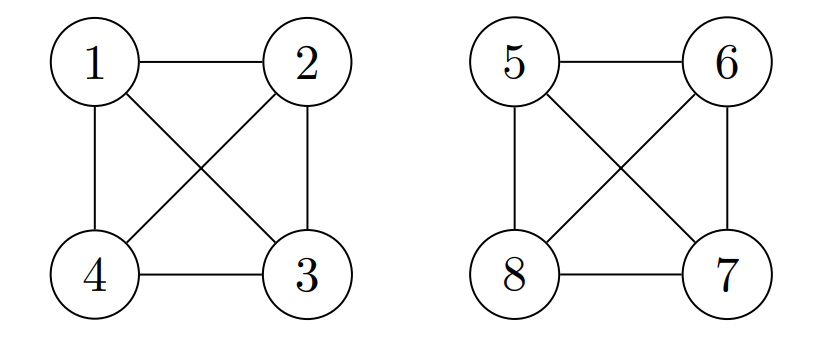
\includegraphics[width=8cm]{1.png}
    \label{fig:node-1}
\end{figure}

There are $\frac{1}{2} \left(\frac{8}{4}\right) = 35$ ways to partition the 8 vertices into two groups of 4, so there are 35 such graphs.
Otherwise, none of 2, 3, 4 are connected to each other. Then 2 and 3 must share a common neighbor, as
must 3 and 4, and 2 and 4. If these are the same neighbor, this vertex would share all three neighbors
with 1, so they must be pairwise distinct. The last vertex must then be connected to these three,
creating a cube graph.

\begin{figure}[H]
    \centering
    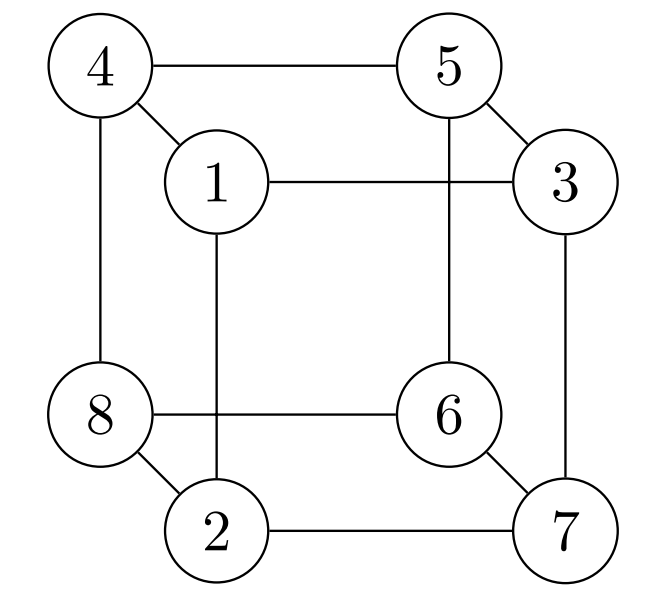
\includegraphics[width=4.5cm]{2.png}
    \label{fig:node-2}
\end{figure}

A cube has 48 symmetries, so the number of such graphs is $\frac{8!}{48} = 840$.\\
The total is 35 + 840 = \boxed{875}.



\end{solution*}


\end{document}